\section{Linear Wave Equation in 3+1 Dimensions with Spherical Symmetry}
\label{sec:spherical_wave}

Next, we need to make our code be able to handle spherical coordinates in 3+1 dimensions with spherical symmetry. This is relevant because many equations (like Einstein's equations) have singularities at the origin of this particular coordinate system.

For that, we will be solving the wave equation in spherical coordinates with spherical symmetry in its PDE system form (equation \eqref{eq:simple_wave_system}), giving the initial conditions

\begin{align}
    \begin{array}{@{}l@{}}
        \Phi(0,x) = e^{-50x^2},
        \\
        \Pi(0,x) = -100e^{-50x^2}.
    \end{array}
    \label{eq:exp_IC}
\end{align}

We will be considering a system of length $L = 5$, imposing that our solution is even on the left boundary, and forcing the solution and its first space derivative to 0 at the right boundary. Even though this treatment at the right boundary is not the most sensible, the boundary is sufficiently far away to not compromise the solution. The goal of this project is not to impose proper boundary conditions.

This time, we will be solving the equation with resolutions of 250, 500, 1000, 2000, and 4000 points, which we combine in pairs and use the same nomenclature as before for the pointwise convergence tests, and then again, also using the previous nomenclature for the norm convergence tests.

The norm convergence of the results and the pointwise convergence as a function of time for the point x = 0 are represented in figures \ref{fig:norm_spherical_wave_2nd_order} and \ref{fig:point_spherical_wave_2nd_order}, while the intensity plot showing the solution is represented in figure \ref{fig:intensity_spherical_wave_2nd_order}.

\begin{figure}[t!]
    \centering
    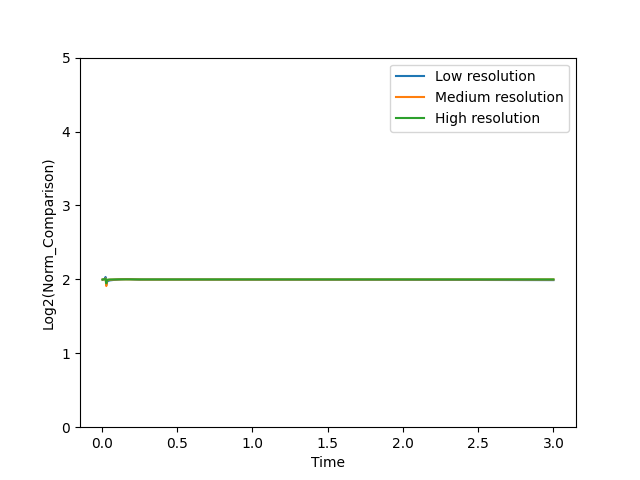
\includegraphics[width=\columnwidth]{Images/spherical_wave-2nd-norm.png}
    \caption{Norm convergence of the solution to the wave equation in 3+1 dimensions with spherical symmetry (with artificial dissipation $\sigma = 0.02$), imposing the parity of the solution at the origin and forcing the wave to 0 at "infinity", while providing initial conditions represented in equation \eqref{eq:exp_IC} in the 2nd-order accurate in space and 1st-order accurate in time code}
    \label{fig:norm_spherical_wave_2nd_order}
\end{figure}

\begin{figure}[t!]
    \centering
    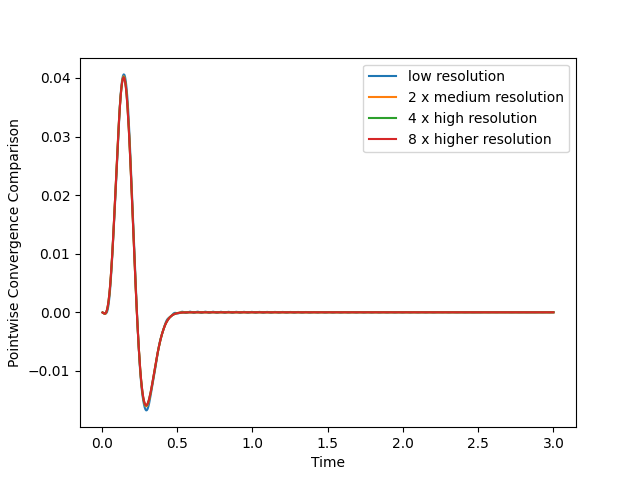
\includegraphics[width=\columnwidth]{Images/spherical_wave-2nd-point.png}
    \caption{Pointwise convergence for $x = 0$ of the solution to the wave equation in 3+1 dimensions with spherical symmetry (with artificial dissipation $\sigma = 0.02$), imposing the parity of the solution at the origin and forcing the wave to 0 at "infinity", while providing initial conditions represented in equation \eqref{eq:exp_IC} in the 2nd-order accurate in space and 1st-order accurate in time code}
    \label{fig:point_spherical_wave_2nd_order}
\end{figure}

\begin{figure}[t!]
    \centering
    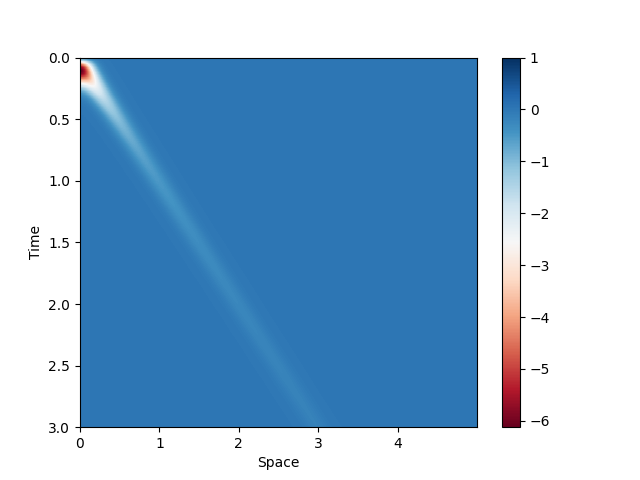
\includegraphics[width=\columnwidth]{Images/spherical_wave-2nd_order-Intensity.png}
    \caption{Intensity plot of the solution to the wave equation in 3+1 dimensions with spherical symmetry (with artificial dissipation $\sigma = 0.02$), imposing the parity of the solution at the origin and forcing the wave to 0 at "infinity", while providing initial conditions represented in equation \eqref{eq:exp_IC} in the 2nd-order accurate in space and 1st-order accurate in time code}
    \label{fig:intensity_spherical_wave_2nd_order}
\end{figure}

On these figures, we can observe a clean convergence again, even though for lower resolutions the convergence at the origin is a little lower. However, this is not worrisome, as that loss of convergence disappears with the increase of resolution.

As previously, this problem was also solved with a 4th-order accuracy in space, and the corresponding results are found in the appendix.

We could also consider the non-linear variant of this equation as we did for 1+1 dimensions. However, we were not able to solve that problem within the time limit of this project, since making the ADM evolution code work was the priority and the principal objective of this project.